\subsubsection{Fletxes d'exploració pels resultats de cerca}

\paragraph{}
S'ha inclòs, just per sobre de la taula de resultats de cerca, una barra de navegació que permet a l'usuari explorar els diferents blocs de persones retornats pel SDK. Recordem, que cada petició retorna un conjunt de quinze persones.

Aquesta barra de navegació consisteix de dues fletxes que permeten navegar endavant i enredera, pels blocs de resultats i un missatge de text que indica quins són els resultats mostrats a la taula, respecte al total de resultats disponibles.

S'ha dotat d’intel·ligència a les fletxes de navegació per assegurar que no s'accedeix a blocs no existents o invàlids.

La imatge~\ref{fig:arrowsPersonSearch} mostra l’aspecte visual d’aquesta funcionalitat.

\begin{figure}[h]
    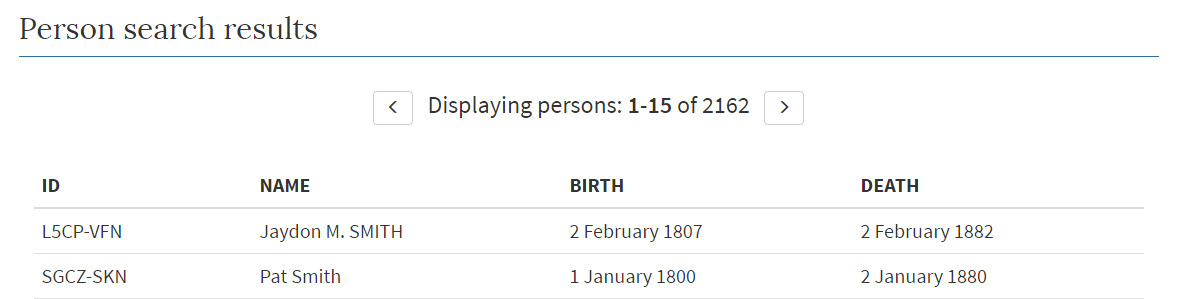
\includegraphics[width=\linewidth]{11/02_searchPersons/06_arrows}
    \centering
    \caption{Fletxes de navegació pels resultats de la cerca a l'arbre familiar}\label{fig:arrowsPersonSearch}
\end{figure}
